% 必须使用PDFLaTeX编译
\documentclass[fontset=windows]{article}
%导言区
%\documentclass{article}%引入一个类【文章的类型】-{或者是book类,有封面;report类;letter类}
\usepackage{texnames}
\usepackage{mflogo}
\usepackage{ctex}
\usepackage{graphicx}
\usepackage{boondox-cal}
\usepackage{boondox-calo}
\usepackage{dutchcal}
\usepackage{mathrsfs}
\graphicspath{{figures/},{graphics/shiyan/}}
%第一种方式就是指定路径,***注意:此文件夹【即graphics文件夹】必须和源文件在同一级目录,,后面的文件夹可以是多级的,***
%\usepackage{xltxtra}
%注:article+use ctex=ctexart
%\usepackage{xeCJK}
%\title{the title of the passage}
%\author{the author}
\title{\LaTeX{} 学习笔记}
\author{\textit{$\mathscr{ZONGPINGDING}$}}
\date{\today}%日期
%正文区   注:一个正文只能有一个document命令
%\newcommand{\myfont}{\text{\textbf{\textsf{Fancy Text}}}}
\begin{document}
    \maketitle
    \tableofcontents 
    %\cite{}
    \section{LaTeX基本命令}
    %\cite{}解决报错没有bib的问题
    %\maketitle    %输出导言区内容作用
    Hello
    %{\songti宋体} \quad
    %hello和公式之间隔一行可以实现分行操作

    $f(x)=x^2+2x-e^x$ %【行内公式】如何输入数学公式;$中间的是数学模式,$之外的是文本模式
    %也可用双$$符号表示公式

    $$f(x)=x^2+2x-3$$

    this is the second polynomial%【行间公式】其会自动换行
    %如何使用中文
    %使用宏包+源文件编码形式为UTF8
    勾股定理可用现代语言表述如下:
    直角三角形斜边的平方等于两腰的平方和
    可以用符号语言表示为:设直角三角形$ABC$,其中$\angle C=90$,则有:
    %我们在此引入了带编号的行间公式环境
    \begin{equation}
        AB^2=BC^2+AC^2.
    \end{equation}
    \section{LaTeX的字体设置}
    LaTeX的字体有五种属性
    \paragraph{1字体编码}
    正文字体编码:OT1T1EU1等
    数学字体编码:OML OMS OMX等
    \paragraph{2字体族}
    罗马字体:笔画起始处有装饰

    无衬线字体:笔画起始处无装饰

    打字机字体:每个字符宽度相同,又称等宽字体;

    下边是演示:

    \textrm{罗马字体 Roman Family}%textsf{}无衬线字体命令 texttt{}打字机字体命令
    %\rmfamily{声明后面字体为罗马字体}%对应上边的几种命令
    \textrm{Roman Family} \textsf{Sans Serif Family} \texttt{TypeWriter Family}
    \rmfamily Roman Family

    jianyan qi'jiezhiqingkuan

    {\sffamily sans serise family} {\ttfamily Typewriter Family}
    %注:这里的{就是罗马family作用的截止处}
    从中我们可以看出有两种方法可以改变字体;
    [1] 字体命令; 使用字体命令作用于\{\}里边的参数

    注:此处我使用了$\backslash$进行转义
    %\的其他输出方法
    %二是: \verb|\|
    %三是:$\setminus$\ 进行转义

    [2] 字体声明; 使用字体命令作用于之后的所有字体,以\{\}为界限

    注: 也可把——family命令的作用范围限制在\{\}里边

    写作\{——family  ……“你的内容”\}

    \paragraph{3字体系列}
    粗细
    宽度

    下边是演示:

    \textmd{medium serise}

    \textbf{Boldface serise}

    对应的\{——family  \}等段落设置略

    注:

    $\backslash$$\backslash$,空行,par(agraph)的区别:

    $\backslash$$\backslash$是换一行顶格开始

    而空一[几行]行,是开启一个新的段落,与par(agraph)作用相同

    务必分清二者的区别


    \paragraph{4字体形状}
    直立
    斜体
    伪斜体
    小型大写

    演示如下:

    \textup{直立字体}

    \textsl{伪斜体}

    \textsc{a b c}

    对比ABC

    对应的字体声明略

    \textit{Italic serise}
    %中文字体

    %{\songti宋体}

    %{\heiti黑体}

    %{\fangsong仿宋}

    %{\kaishu楷书}
    %中文字体的斜体,粗体
    注:中文的斜体是用楷书表示的
    \paragraph{5字体大小}
    %可在文档的开头设置文章字体的大小

    %格式为documentclass[10pt]{article},此时是10磅 注:只有10 11 12磅
    %另外ctex宏包里边还有 格式:zihao{3}+ 内容
    %之后的文字的“大”和“小”都是相对于文档开始字体的大小的
    %集体命令有
    {\tiny Hello}

    {\scriptsize Hello}

    {\footnotesize Hello}

    {\small Hello}

    {\normalsize Hello}

    {\large Hello}

    {\LARGE Hello}

    {\huge Hello}

    {\Huge Hello}

    \textbf{最重要的,可以在begin之前自定义命令}

    演示如下:

    \paragraph{6篇章结构}
    \textbf{生成目录}

    %使用\tableofcontents命令
    %\chapter{绪论}
    \section{国内研究现状}
    \section{研究此实验的现实意义}
    %\chapter{实验与结果分析}
    \section{引言}
    \section{实验方法}
    \section{实验结果}
    \subsection{数据}
    \subsection{图表}
    \subsubsection{图表1}
    \subsubsection{图表2}
    \subsection{结果分析}
    \section{实验的反思}
    %注:subsubsection会与chapter冲突
    \paragraph{\LaTeX{} 中的特殊字符的学习}

    \section{空白符号}
    空行分段,多个空行等于一个

    自动缩进,不能用空格代替

    英文中多个空格等于一个空格,中文中空格会被忽略

    汉字与其他字符的间距会自动由XeLaTeX处理

    不能还用中文全角空格

    若要输出空白则用:\\
    a\quad b\\
    %注;yi一个quad相当于当前字体的M宽度,1em
    a\qquad b\\
    %2em
    a\,b or a\thinspace b\\
    %1/6em,转义字符
    a\enspace b\\
    %0.5em
    a\ b\\
    %注:此时是\加一个空格
    a~b\\
    %硬空格,不能分割
    指定间距\\
    a \kern 1pc b\\
    a\kern -1em b\\
    %负值说明顺序不同
    a\hskip 1em b\\
    a\hspace{35pt}b\\
    a\hfill b\\
    %弹性长度空白
    注:1pc=12pt=4.218mm
    \section{\LaTeX{} 控制符}
    %实际上就是转义字符\\
    \section{排板符号}
    \textbf{重要}

    \S \P \dag \ddag \copyright \pounds
    \section{\TeX{} 标志符号}
    \LaTeX{} \TeX{} \LaTeXe{} %\XeLaTeX
    \section{引号}
    单引号左右。双引号左右\\
    `'``''``你好''
    \section{连字符}
    - -- ---
    \section{非英文字符}
    \oe \OE  \aa \AA
    \section{重音字符(以o为例)}
    \section{\LaTeX{} 里边的插图}
    \section{重音字符(以o为例}

    \section{\LaTeX{} 里边的插图}
    \textbf{使用格式}

    导言区使用$\backslash$usepackage{graphicx}和

    $\backslash$graphicspath\{\{文件的路径,比如:文件夹1$/$\},\{文件夹2\}\}

    正文区使用语法:$\backslash$includegraphics[选项]{文件名}

    格式:EPS PDF PNG JPEG BMP

    实例如下:

    调节图片的几种方法如下:

    \includegraphics[width=3in,height=4in,keepaspectratio]{ghost}
    %\caption{figure one}
    %这里不能用caption命令

    
\includegraphics[angle=45,height=8cm,keepaspectratio]{girl}
    %不同参数之间用,分割
    %\caption{figure two}

    \includegraphics[scale=0.03]{ghost}
    %\caption{figure three}

    \includegraphics[height=0.1\textheight]{ghost}
    %\caption{figure four}
    %第二种方法

    \begin{figure}
        \centering
        
\includegraphics[scale=0.5]{{graphics/shiyan/girl}}
        \caption{figure five}
        %\label{fig:_my label}
        %注:此处的注释的Lable最好放在最后面,即end的前边
    \end{figure}
    \section{表格的制作}

    \begin{tabular}{|l|| c| c| c |r|}%对齐方式:左 中 右 用|产生表格竖线,双竖线
        \hline \hline
        %\hline 用以产生横线,双横线
        姓名&语文&数学&英语&体育\\%不同列之间用&连接,用\\结束本行
        \hline
        张三&78&56&45&100\\
        \hline
        李四&21&94&75&90\\
        \hline
        王五&48&96&45&77\\
        \hline 
    \end{tabular}
    \section{图片,表格的浮动}%意思就是图片,表格等都处在文字的上边

    \LaTeX{} 中的插图见图\ref{fig-falling}

    \begin{figure}[htbp]%注:用这一可选参数控制了浮动体的位置
        \centering%注:centering的意思是让环境中的内容居中排版
        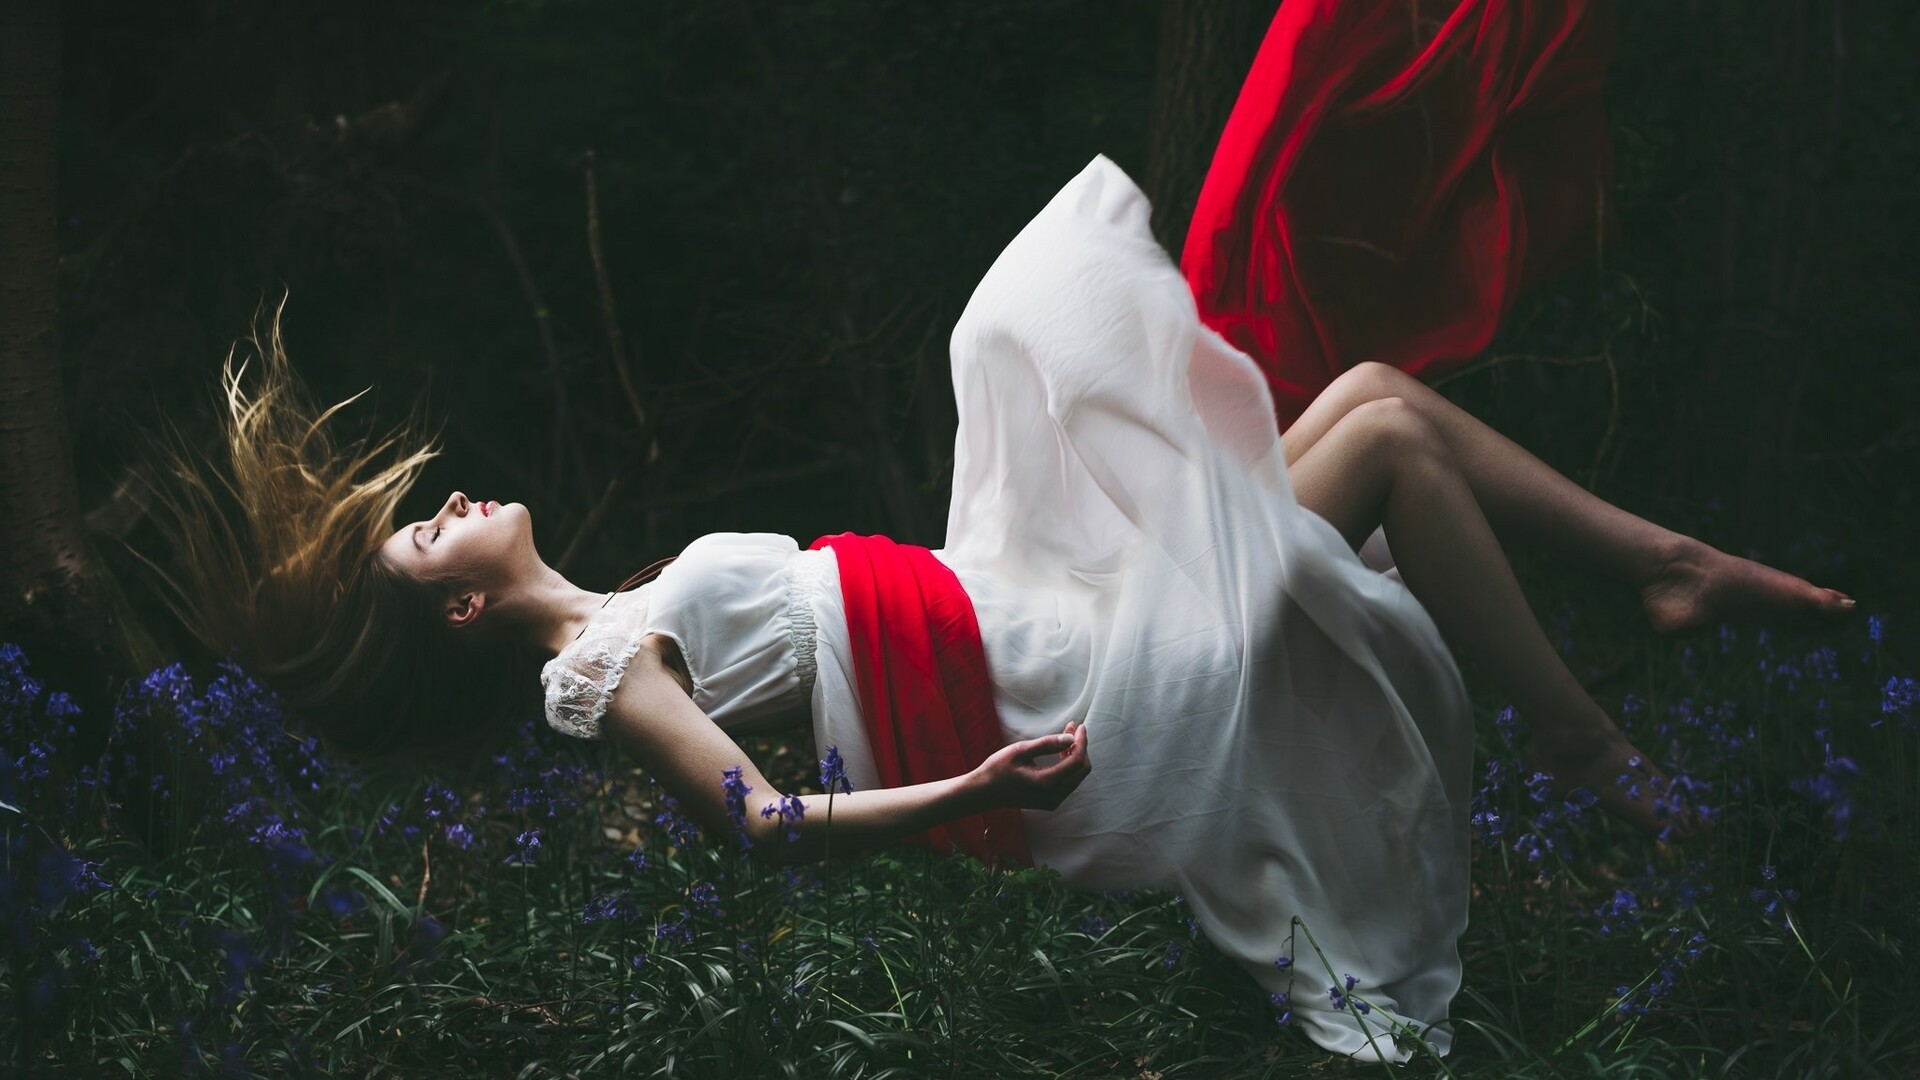
\includegraphics[scale=0.2]{{graphics/falling}}
        \caption{figure five}
    \end{figure}

    \LaTeX 中的表格,见表

    \begin{table}
        \centering
    \begin{tabular}{||l| c| c| c |r|}%对齐方式:左 中 右 用|产生表格竖线
        \hline \hline
        %\hline 用以产生横线
        姓名&语文&数学&英语&体育\\%不同列之间用&连接,用\\结束本行
        \hline
        张三&78&56&45&100\\
        \hline
        李四&21&94&75&90\\
        \hline
        王五&48&96&45&77\\
        \hline
    \end{tabular}
    \caption{考试成绩}
    \end{table}

    \section{附录:花体英文}
    见以下实例:
    $$\mathcal{ABCGEFGHIJKLMNOPQRSTUVWXYZ}$$

    $$\mathcal{abcdefghijklmnopqrstuvwxyz}$$

    $$\mathbcal{ABCGEFGHIJKLMNOPQRSTUVWXYZ}$$

    $$\mathbcal{abcdefghijklmnopqrstuvwxyz}$$

    $\mathscr{ABCGEFGHIJKLMNOPQRSTUVWXYZ}$

    \textit{$\mathcal{ABC}$}

    \textit{$\mathscr{ABC}$}

    \label{fig:_my label}
    \label{fig-falling}%给浮动体设置的标签
        %注意:这里标签的格式为 fig-名称
\end{document}

